\section{停留时间分布的实验测定}


\begin{frame}
    \frametitle{脉冲法}

    在极短的时间内、在系统入口处向流进系统的流体加入一定量的示踪剂，输入示踪剂后，立刻检测系统出口处流体中示踪剂浓度随时间的变化。
    \vspace{-4pt}
    \begin{figure}
        \centering
        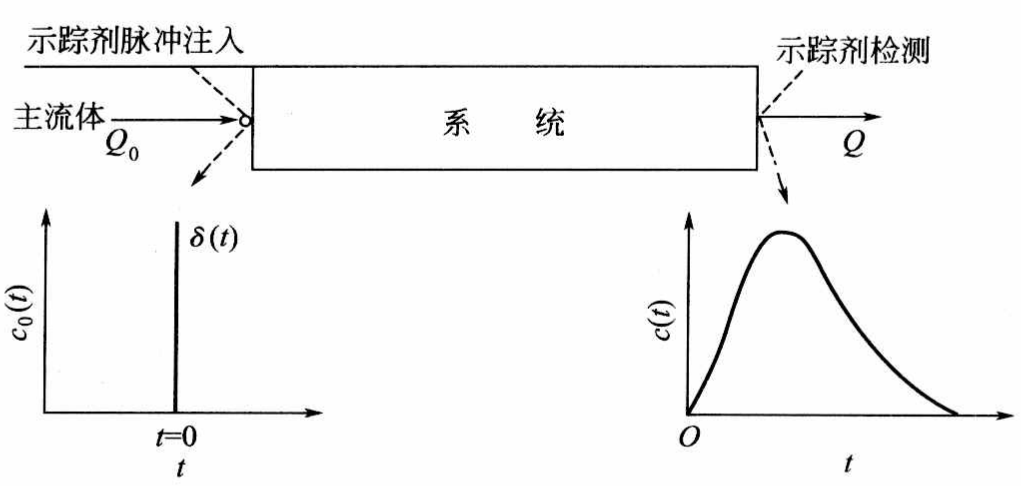
\includegraphics[width=.55\linewidth]{figures/fig5.5.png}
    \end{figure}
    \vspace{-7pt}
    \begin{blankblock}{}
        狄拉克$\delta$函数是一个广义函数，在物理学中常用其表示质点、点电荷等理想模型的密度分布，该函数在除了零以外的点取值都等于零，而其在整个定义域上的积分等于1。
    \end{blankblock}

\end{frame}
% 物理学中常常要研究一个物理量在空间或时间中分布的密度，例如质量密度、电荷密度、每单位时间传递的动量（即力）等等，但是物理学中又常用到质点、点电荷、瞬时力等抽象模型，他们不是连续分布于空间或时间中，而是集中在空间中的某一点或者时间中的某一瞬时，那么它们的密度应该如何表示呢？
% 上述表达式不规定δ函数在0点的取值，是因为这个值无法严谨地表述出来，不能笼统的定义为正无穷，并且函数取值的“大小”是由第二个积分式决定的，因此只需限定取值为零的区域即可。


\begin{frame}
    \frametitle{脉冲法}

    根据$E(t)$的定义得
    \[
        Q c(t) \mathrm{d} t=m E(t) \mathrm{d} t
    \]
    \[
        E(t)=\frac{Q c(t)}{m}
    \]
    $m$为加入示踪剂的量（mol）。

    当示踪剂的量不能准确知道时，可通过下式计算：
    \[
        m=\int_{0}^{\infty} Q_{c}(t) \mathrm{d} t
    \]
    \[
        E(t)=\frac{c(t)}{\int_{0}^{\infty} c(t) \mathrm{d} t}
    \]

\end{frame}


\begin{frame}[t]
    \frametitle{}

    \begin{example}
        流化床催化裂化装置中的再生器，其作用系用空气燃烧硅铝催化剂上的积炭使之再生。进入再生器的空气流量为\SI{0.84}{kmol.s^{-1}}现用氦气作示踪剂，采用脉冲法测定气体在再生器中的停留时间分布，氦的注入量为\SI{8.84e-3}{kmol}。试求$t=35s$时的停留时间分布密度和停留时间分布函数。
        \begin{table}[]
            \caption{再生器出口气体中氦的浓度$c$（用氦与其他气体的摩尔比表示）和时间的关系}
            \begin{tabular}{l|lllllllll}
            \hline
            $t/s$ & 0 & 9.6 & 15.1 & 20.6 & 25.3 & 30.7 & 41.8 & 46.8 & 51.8 \\ \hline
            $c \times 10^6$ & 0 & 0 & 143 & 378 & 286 & 202 & 116 & 73.5 & 57.7 \\ \hline
            \end{tabular}
            \end{table}
    \end{example}

\end{frame}


\begin{frame}
    \frametitle{阶跃法}

    \begin{itemize}
        \item 升阶法
        
        将在系统中作定常流动的流体切换为流量相同的含有示踪剂的流体
        \item 降阶法
        
        将在系统中作定常流动的含有示踪剂的流体切换为流量相同的不含示踪剂的流体
    \end{itemize}

    \begin{figure}
        \centering
        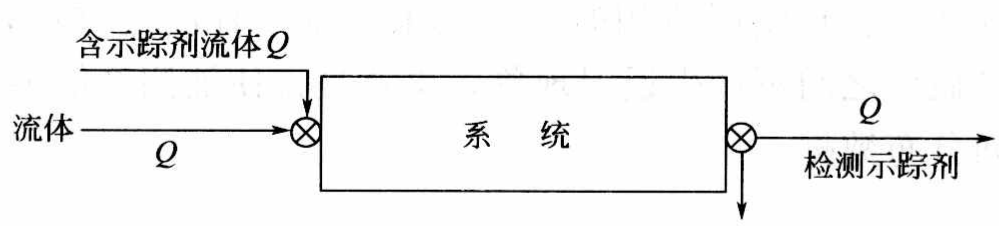
\includegraphics[width=.9\linewidth]{figures/fig5.6a.png}
    \end{figure}

\end{frame}


\begin{frame}
    \frametitle{升阶法}

    \begin{figure}
        \centering
        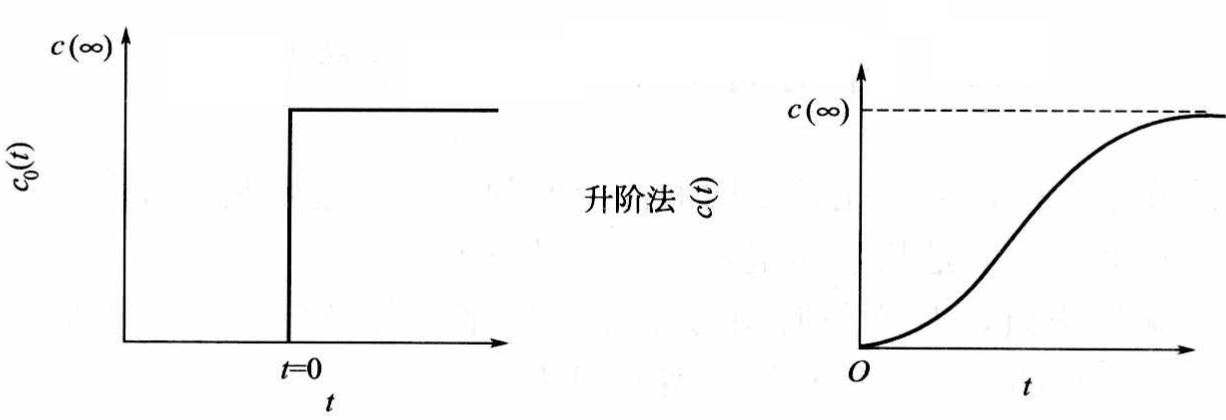
\includegraphics[width=.9\linewidth]{figures/fig5.6b.png}
    \end{figure}
    \begin{minipage}{0.48\linewidth}
        输入的阶跃函数

        $c_0(t) = 0 \qquad (t<0)$
        
        $c_0(t) = c(\infty)=\text{常数} \qquad (t\geqslant 0)$
    \end{minipage}\hfill
    \begin{minipage}{0.48\linewidth}
        \[
        F(t) = \frac{Qc(t)\dif t}{Qc(\infty)\dif t} = \frac{c(t)}{c(\infty)} = \frac{c(t)}{c(0)}
        \]
    \end{minipage}

\end{frame}


\begin{frame}
    \frametitle{降阶法}

    \begin{figure}
        \centering
        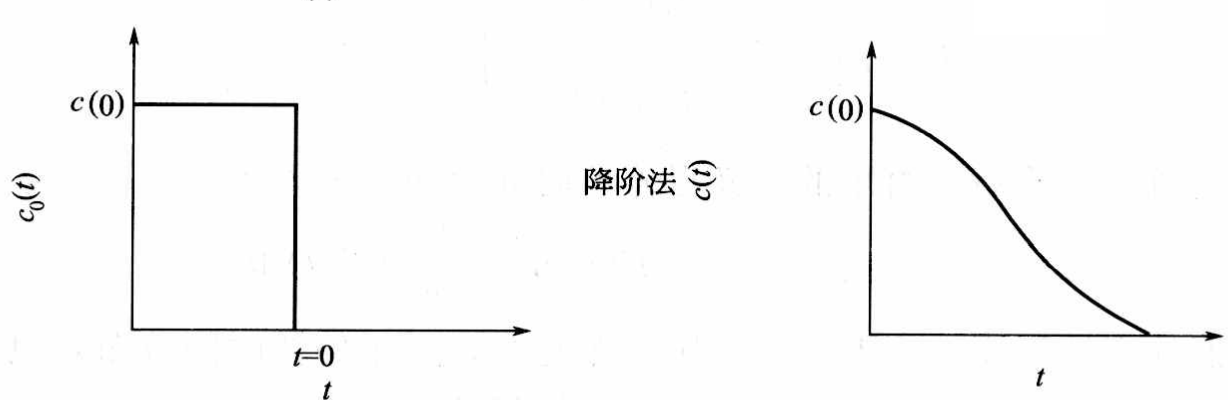
\includegraphics[width=.9\linewidth]{figures/fig5.6c.png}
    \end{figure}
    \begin{minipage}{0.48\linewidth}
        输入的阶跃函数

        $c_0(t) = c_0 =\text{常数} \qquad (t<0)$
        
        $c_0(t) = 0 \qquad (t\geqslant 0)$
    \end{minipage}\hfill
    \begin{minipage}{0.48\linewidth}
        $c(t)/c(0)$为停留时间大于$t$的物料所占的分数
        \[
        1 - F(t) = c(t)/c(0)
        \]
    \end{minipage}

\end{frame}


\begin{frame}
    \frametitle{选择示踪剂的原则}

    \begin{enumerate}
        \item 示踪剂不与主流体发生反应；
        \item 示踪剂应当易于和主流体溶为（或混为）一体，除了显著区别于主流体的某一可检测性质外，两者应具有尽可能相同的物理性质；
        \item 示踪剂浓度很低时也能够容易进行检测，这样可使示踪剂用量减少而不致影响主流体的流动；
        \item 示踪剂的浓度与要检测的物理量的关系应有较宽的线性范围，以便直接利用实验测定数据进行计算而不必再作校正和变换；
        \item 用于多相系统的示踪剂不发生从一相转移到另一相的情况，例如，气相示踪剂不能被液体所吸收，而液相示踪剂也不能挥发到气相中去；
        \item 示踪剂本身应具有或易、于转变为电信号或光信号的特点，从而能在实验中直接使用现代仪器和计算机采集数据作实时分析，以提高实验的速度和数据的精度。
    \end{enumerate}

\end{frame}


\begin{frame}
    \frametitle{脉冲法/阶跃法的比较}

    \begin{table}[]
        \caption{脉冲法/阶跃法的优缺点}
        \begin{tabular}{l|cc}
        \hline
         & 优点 & 缺点 \\ \hline
        脉冲法 & \makecell{示踪剂消耗量少 \\ 可直接求出$E(t)$} & 如何使示踪剂的输入时间缩到最短 \\ \cline{2-3} 
        阶跃法 & 容易操作 & \makecell{示踪剂用量较多 \\ 直接求出的是$F(t)$} \\ \hline
        \end{tabular}
        \end{table}
        在实际应用时，无论采用哪一种测定方法，都必须保证在示踪剂输入点与系统入口截面之间不产生返混现象，也就是说使被测系统为闭式系统，这样才可获得准确的停留时间分布数据。

\end{frame}
